
\chapter{SECURITY TEST FRAMEWORK}

Architecture for Security test framework is depicted in Figure 7.1. It has been implemented in python using requests library and mechanize browser[8] through an API. Requests are used to send http requests and acquire responses from web applications. Mechanize is a Stateful and headless web browser. Headless web browser or UI less web browser is suited for our purpose because in some cases of browsers with UI like chrome or firefox, browser side security can prevent the security attacks while the web application is still vulnerable to security. Such kind of attacks is made possible in headless browser and it is identified in our experimentation. 

\begin{figure}[htpb]
 \begin{center}
    \resizebox{150mm}{50mm} {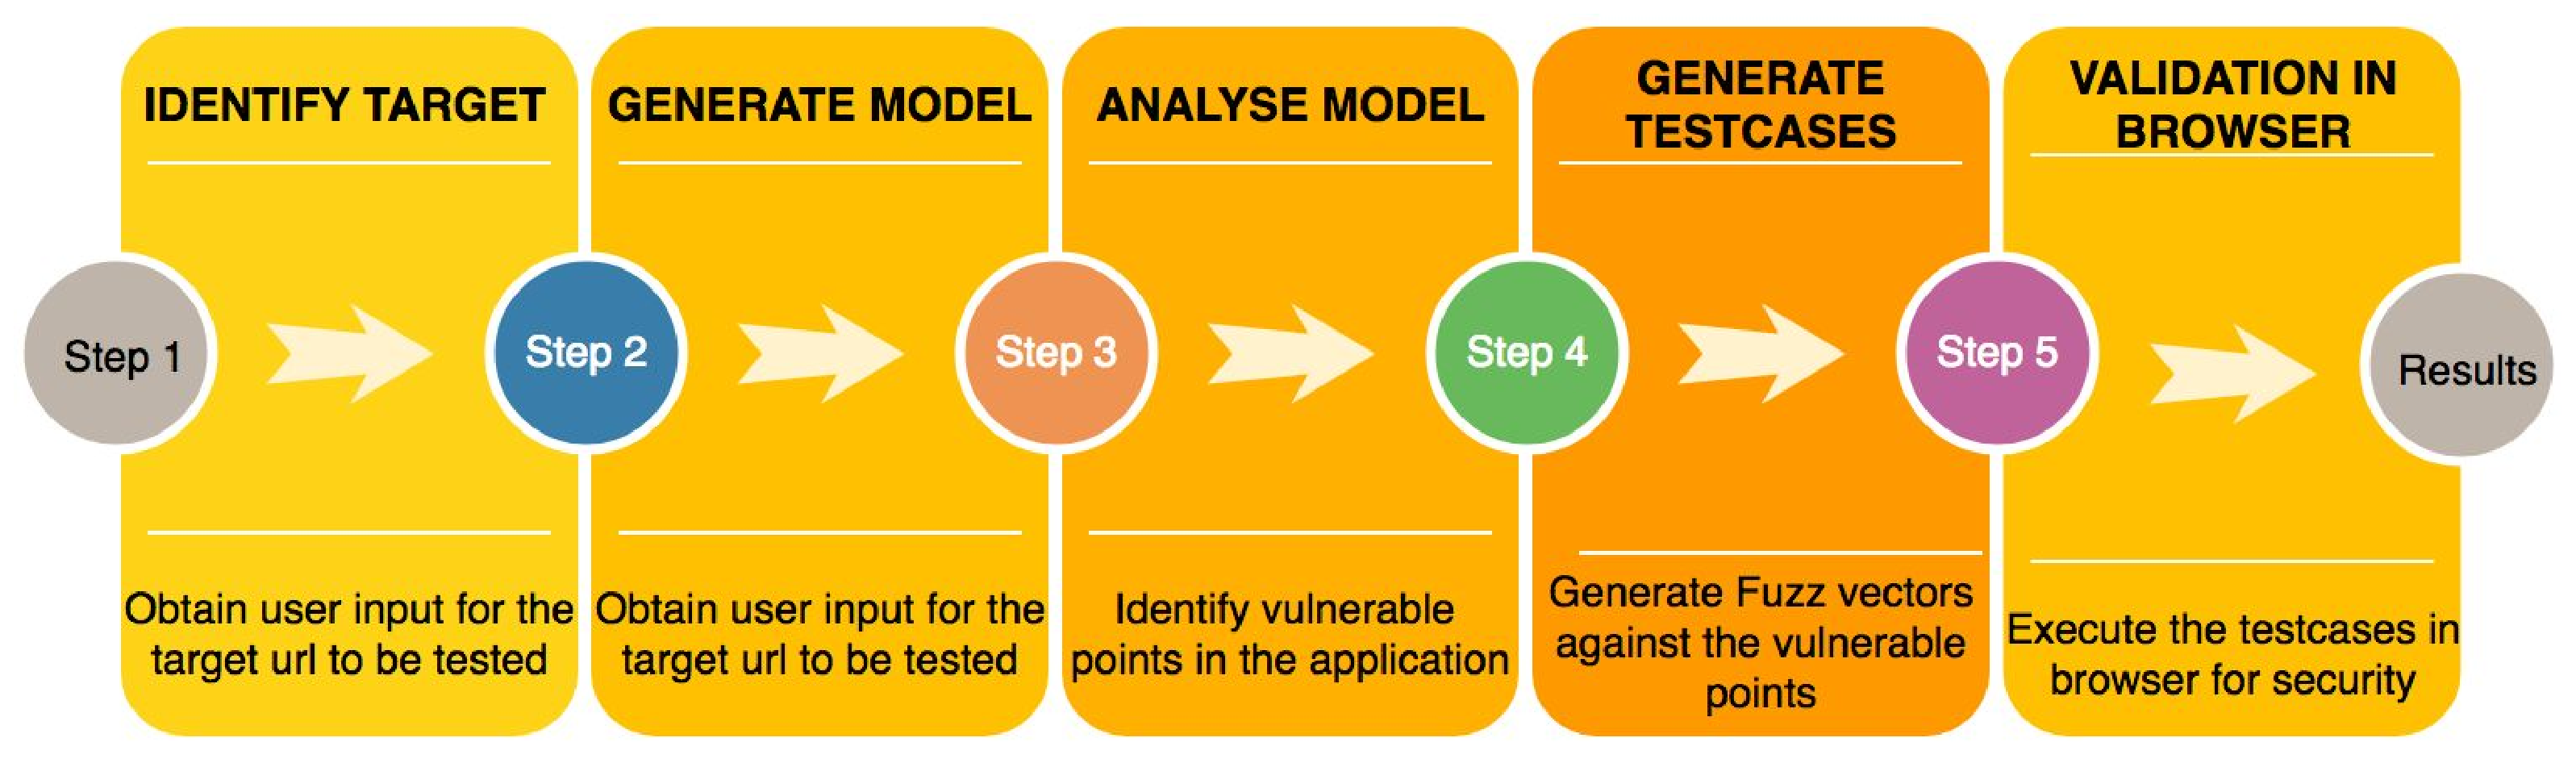
\includegraphics {Chapters/architecture1.eps}}
    \caption {Architecture}
  \label{fig:Table}
 \end{center}
\end{figure}

\section{Identification of Vulnerable points of attack from the model}
The State machine model represents the architecture and the DOM elements of the the web applications. The next step is to define the attack pattern and test objective of Security Testing. The most vulnerable security threats are XSS and SQLI attacks. The candidate elements such as forms fields, user inputs, GET and POST parameters which are vulnerable to these attacks are determined from the the DOM tree extracted in the State Machine model as follows. 
\\
DOM tree of the start state is obtained from the state machine. Tags in the DOM Tree are parsed only by one and user modifiable elements are captured.
Form fields, user inputs, GET/POST parameters and textarea fields, are identified added to a list named as vulnerable elements. Form fields are identified with their tag attribute id. Both the form name and id attributes are added to the list. User Input fields, password field are identified with their tag attribute name. If tag attribute id is not present then tag attribute name is used for input fields identification. Input Elements whose element those are hidden in the web page are also added to the vulnerable elements. All the fields identified as vulnerable elements are stored in a file Vulnerability\_model.
If there are no user modifiable fields, then there are no candidate elements are found for vulnerability for that particular DOM state. The DOM state is marked as visited and the process is repeated for all states in the state machine.. The vulnerability\_model is output to the user as HTML report for all the states.
This analysis is implemented by a parsing the DOM Tree using Beautifulsoup library[9]. \\

Example of Vulnerable fields identified from model;\\

 \\$<input class="loginInput" name="username" size="20" type="text"/>$

 \\$<input autocomplete="off" class="loginInput" name="password" size="20" type="password"/>$

 \\$<input name="Login" type="submit" value="Login"/>$

\section{Test Suite Generation based on the Model}

The vulnerability points are tested for XSS Attacks and SQL Injection attacks. The test cases are generated for these vulnerability points using the following methods.

\subsection{Test Suite Generation for XSS Attack}

Consider a simple model with a webpage having a input element such a search box and a submit button which displays the results of a search query. \\

The webpage http://www.xssgame.com/f/m4KKGHi2rVUN/ is show as below:

\begin{figure}[!h]
 \begin{center}
    \resizebox{100mm}{75mm} {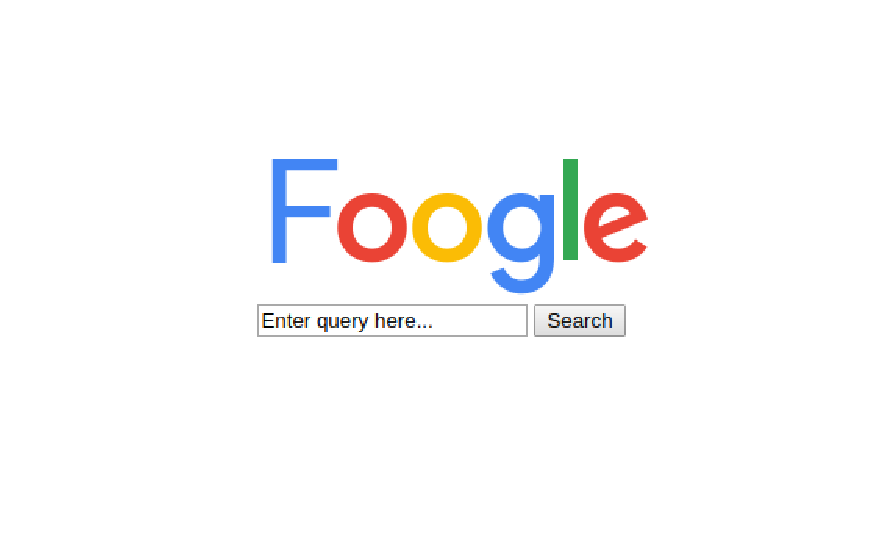
\includegraphics {Chapters/XSS.eps}}
    \caption {Test Webpage for XSS Attack}
  \label{fig:Table}
 \end{center}
\end{figure}

The test case for XSS attack is derived from the model as follows. \\
State Tested: Start State \\
Target Element: Search Input Box (identified from model)\\
$
<input id="demo2-query" name="query" onfocus="this.value=''" value="Enter query here..."/>$\\
$<input id="demo2-query" name="query" onfocus="this.value=''" value="Enter query here..."/>
$\\
Attack Script: $<script>alert('XSS')</script> $\\
\newline
If the XSS script gets reflected as $<SCRIPT>alert('XSS');</SCRIPT> $ in HTTP Response then the attack has succeeded. This implies there is no filters or input sanitization performed for the attack script. The javascript is executed by the browser.\\
Instead, it it gets displayed as$ &lt;SCRIPT&gt;alert('XSS')</SCRIPT&gt;$ then the attack is not successful, since the special characters of script are escaped and encoded. The javascript will not be executed by the browser.
Similarly the test cases are generated for multiple states, target elements and attacks scripts. The testcases are variants of javascript, execution of javascript embedded in different tags like body, img src. Javascript codes to escape the filters of web application are also part of test cases.
\\
There are two variants of XSS attacks, Persistent or Stored XSS and Non-persistent or Reflected XSS attacks. 
\\
In Non-persistent or reflected XSS attack, the javascript is injected to the user accessing web application but the script is not stored in the web application permanently. For this kind of attack after injecting the code, the resulting HTTP response is verified.
\\
In persistent of stored XSS attacks, the javascript is stored permanently in the database of the web application and the script is executed for all persons who access the web application. For persistent XSS attack, after injecting the script, the HTTP response should be verified and also web application should be loaded again and checked whether the malicious script is loaded. This kind of attack happens when image comment is stored in a web application, or a message is posted in a forum.
\\
Example XSS Attack testcases.
\\
$ <BODY ONLOAD=alert('XSS')>$\\
$<IMG SRC="javascript:alert('XSS')"$\\
$</xmp><script>alert(‘XSS’)</script><xmp>$\\
$<SCRIPT/SRC="http://xss.rocks/xss.js"></SCRIPT>$

\subsection{Test Suite Generation for SQLI Attack}

The objective of SQLI inject testing is to read unauthorized stored data from a database at the back end of web application such as passwords and usernames. The test suite for SQLI attack is generated by deriving SQL queries for retrieving stored data.  The first phase is to find which all input parameters which will flow into the SQL query Statements. These are the SQL queries which are vulnerable to SQLI attacks. Example of input fields are username and password field which which will be translated as a SQL query to validate credentials in the database. The target input fields vulnerable to SQLI attacks are extracted from the State graph model. \\

Consider a web page having input elements such a username and password fields.

\begin{figure}[!h]
 \begin{center}
    \resizebox{100mm}{75mm} {\includegraphics {Chapters/SQLI.eps}}
    \caption {Test Webpage for SQLI Attack}
  \label{fig:Table}
 \end{center}
\end{figure}


\\
The sample test case for SQL Injection attack is as follows. 
\\
State Tested: Root DOM State (identified from state machine)\\
Target Element: password Field  (identified from state machine)\\
$
<input class="loginInput" name="username" size="20" type="text"/>$\\
$<input autocomplete="off" class="loginInput" name="password" size="20" type="password"/>$
\\
Attack SQL Query: 1 OR 2=2\\
\newline
Entering a username and password into the query will flow into the database as USERNAME="uname" and PASSWORD="pwd". With the attack SQL Query 1 OR 2=2. SQL Query will flow as USERNAME="uname" and PASSWORD="1" OR 2=2.
If the web application does not have security measures to control the attack the password check will be bypassed and application will login. If the resulting response contains invalid password then the attack is successful else the password check is bypassed and attack is successful.
\\
\newline
Similarly the test cases are generated for all the states, target elements and SQL Injection queries.
\\
\newline
Example SQL Injection Attack testcases.\\
$‘TEST$\\
$SELECT VERSION();$\\
$1' OR '1'='1$\\
$1'1$\\
$1 AND 1=1$\\
$1' AND 1=(SELECT COUNT(*) FROM tablenames); --$\\
$1' AND non_existant_table = '1$\\
$OR username IS NOT NULL OR username = '$\\

 \\
\section{Fuzzing Based Techniques for Test Suite Generation}

Fuzz Testing is a software testing technique in which invalid or random generated data called fuzz is created. In our tool, the attack vectors are generated using The steps for fuzz testing include the basic testing steps. The steps for fuzz testing include the basic testing steps-

\begin{itemize}
\item Identify the target DOM State.
\item Identify GET/POST parameters and user input fields vulnerable to security flaws
\item Generate Fuzzed attack vectors using recursive fuzzing, bruteforce fuzzing and replacive fuzzing techniques.
\end{itemize} 

We employ replacive fuzzing by replacing the special characters which can be escaped by their hexadecimal codes. Replacive fuzzing is employed by changing the user modifiable parameters reflected in the URLs of states in the state machine.

\section{Validation of the attack pattern from model in Browser}

 The target parameters and testcases are derived from the model as explained in above sections. 

Target parameters:

$
<input id="demo2-query" name="query" onfocus="this.value=''" value="Enter query here..."/></xmp>$\\
$<input id="demo2-query" name="query" onfocus="this.value=''" value="Enter query here..."/>$
\\
$
<input class="loginInput" name="username" size="20" type="text"/>
<input autocomplete="off" class="loginInput" name="password" size="20" type="password"/>
$
 
XSS Attack testcases.
\\
$ <BODY ONLOAD=alert('XSS')>$\\
$<IMG SRC="javascript:alert('XSS')"$\\
$</xmp><script>alert(‘XSS’)</script><xmp>$\\
$<SCRIPT/SRC="http://xss.rocks/xss.js"></SCRIPT>$\\
\newline
SQL Injection Attack testcases.\\
$‘TEST$\\
$SELECT VERSION();$\\
$1' OR '1'='1$\\
$1'1$\\
$1 AND 1=1$\\
$1' AND 1=(SELECT COUNT(*) FROM tablenames); --$\\
$1' AND non_existant_table = '1$\\
$OR username IS NOT NULL OR username = '$\\
 \newline
The execution framework is implemented in python using Requests Library and Mechanize browser. Mechanize is a headless browser, browser without UI and it is suited for our purpose because browsers like firefox, chrome has security mechanisms implemented with them and they can block attack scripts and provide false negatives. But the web application may be still vulnerable to security attacks. Requests library is used to load content from the web application, the requested content is intercepted. The target parameters identified from the model are now injected with malicious scripts from testcases in the intercepted content. Browser object is created for mechanize browser. The intercepted content is now submitted to the mechanize browser using the browser object created.\\
\newline
The resulting HTTP response from the web application is stored in a debug.log file. The resulting HTTP response from the debug.log file is now analysed whether the injected script is executed. If the HTTP Response contains the injected javascript without filters then it implies the reflected XSS attack is possible.  If the elements cannot be modified, the response is obtained as the element is read only. This implies the attack is not successful. For stored XSS attack, after injecting the script, open the browser web application again through a different browser object and find whether the web application contains the injected code. For SQL Injection attacks, if the resulting HTTP response contains data from the web application database, the attack is successful. For malformed SQL queries, if the HTTP response contains any syntax error or database error or database version is obtained, the attack is successful since the SQL query gets executed is not filtered by the web application. If the SQL query is not executed and if the HTTP response contains invalid input, attack is not successful.\\

The output obtained is written into a summary file for all the states whether the attack is successful or not.
 

\\In the next chapter, we shall illustrate our framework with a CASE study.
